\begin{subsectionframemod}{Cross-Domain Few-Shot Object Detection}
    \metroset{block=fill}
    \vspace{-10mm}
    \begin{alertblock}{Détection d'objet few-shot cross-domain}
        Dans la détection d'objets à faible échantillon inter-domaines (CD-FSOD), deux ensembles de données distincts sont utilisés pendant l'entraînement de base et l'affinage.
        La CD-FSOD est plus difficile, car le modèle doit non seulement s'adapter à de nouvelles classes, mais aussi à de nouvelles images.
    \end{alertblock}
    \vspace{5mm}

    \only<1>{
        \begin{figure}
            \centering
            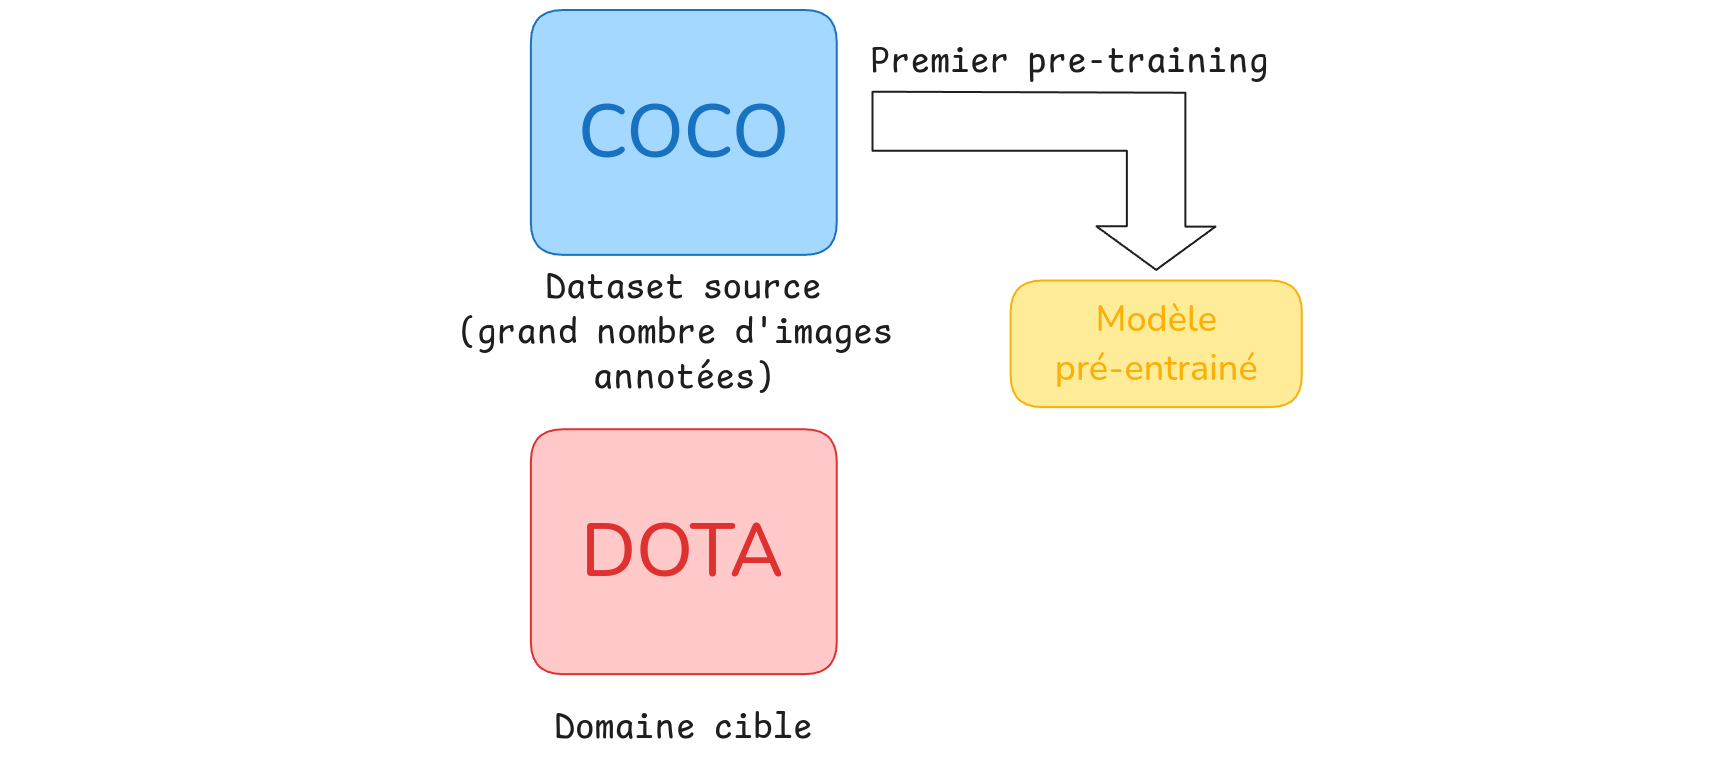
\includegraphics[width=0.6\textwidth]{Figures/cross_domain_1}
        \end{figure}
    }
    \pause
    \only<2>{
        \begin{figure}
            \centering
            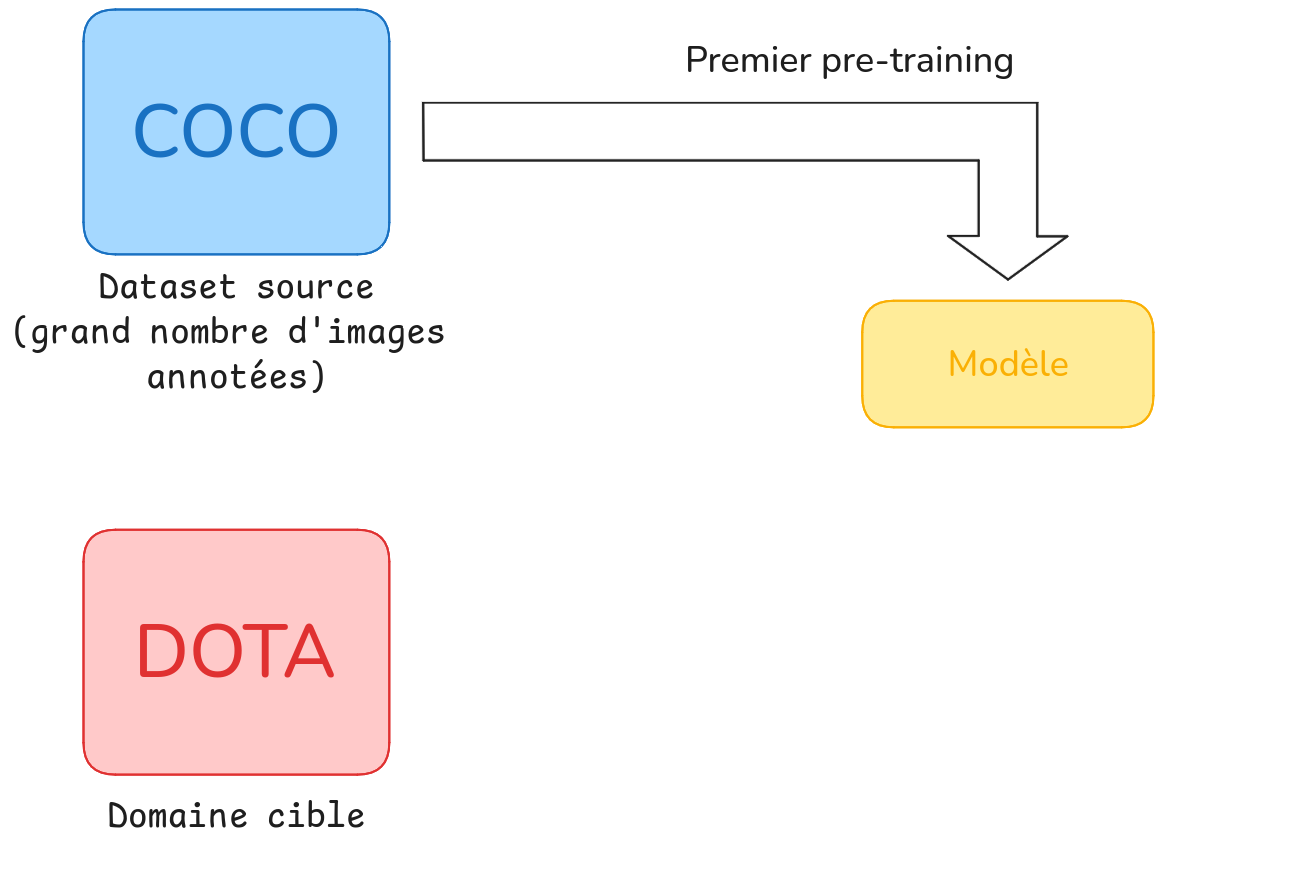
\includegraphics[width=0.6\textwidth]{Figures/cross_domain_2}
        \end{figure}
    }
    \pause
    \only<3>{
        \begin{figure}
            \centering
            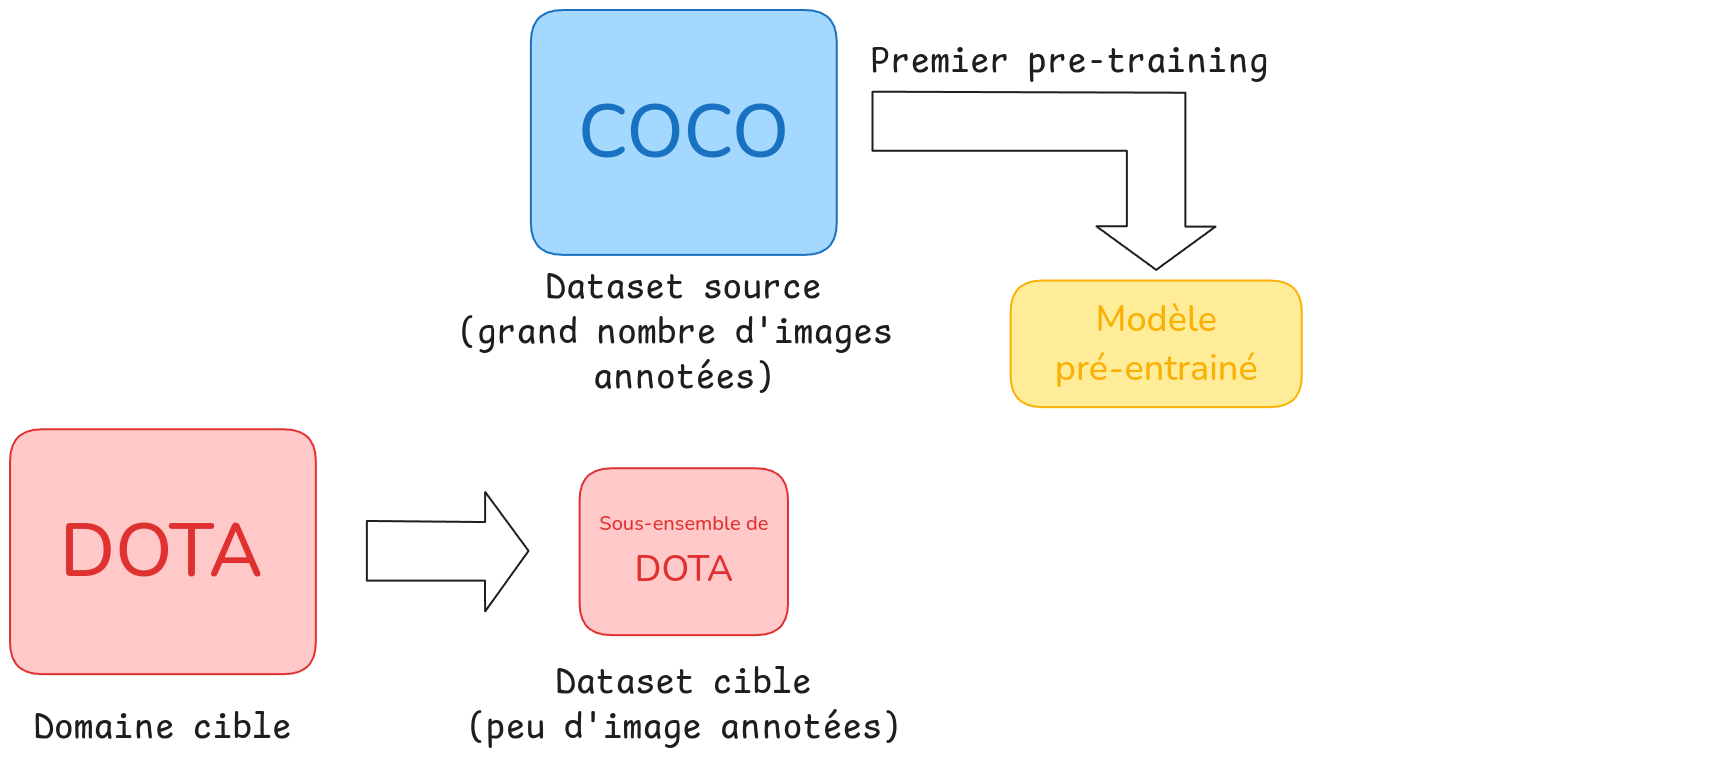
\includegraphics[width=0.6\textwidth]{Figures/cross_domain_3}
        \end{figure}
    }
    \pause
    \only<4>{
        \begin{figure}
            \centering
            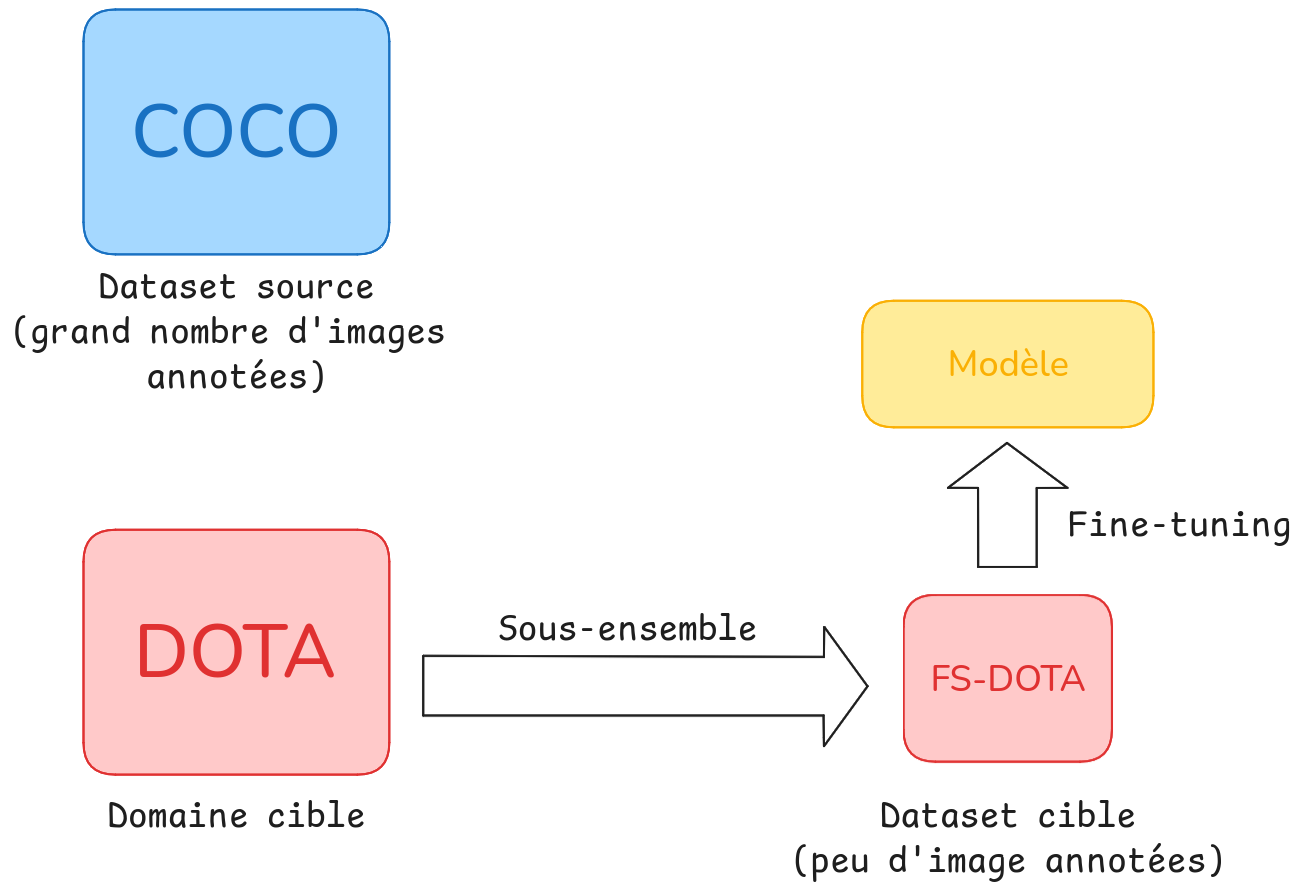
\includegraphics[width=0.6\textwidth]{Figures/cross_domain_4}
        \end{figure}
    }

\end{subsectionframemod}